\documentclass[
  journal=largetwo,
  %manuscript=review,
  year=2025,
  volume=37,
]{cup-journal}

\input{preamble.tex}
\input{math_commands.tex}

\addbibresource{references.bib}

\title{Polynomial, neural double descent and the component perspective}

\author{Bui Gia Khanh}
\affiliation{Department of Physics, Hanoi University of Science, Vietnam National University, Hanoi Vietnam}
\email[Bui Gia Khanh]{fujimiyaamane@outlook.com}

\author{Luong Van Tam}
\affiliation{Department of Physics, Hanoi University of Science, Vietnam National University, Hanoi Vietnam}
% \alsoaffiliation{Joint first authors}

\author{Dang Tri Trung}
\affiliation{Monash University, Department of Computer Science, Melbourne, Australia}

\author{Daud Shahbaz}
\affiliation{COMSATS University Islamabad, Islamabad, Pakistan}

%\addbibresource{references.bib}

\keywords{Statistical learning theory, double descent, deep learning, computational complexity theory, complexity theory, grokking} %% First letter not capped

\begin{document}
\begin{abstract}
    The analysis of learning action, machine learning and related practices in the field theoretically has been made by utilizing Computational Learning Theory (CoLT) \cite{10.1145/1968.1972} and Statistical Learning Theory (SLT) \cite{Vapnik1999-VAPTNO}. These two theories, while overlapped, provides a general framework in analysing and justifying learning actions and learning model constructions, aiding in the formation of modern practices. One of the famous insight using such framework is the \textit{bias-variance tradeoff} \cite{6797087}, which states that model complexity and generality inversely affect each other, thus guarantee the need for a safe bracket between them. However, recent literatures, \cite{belkin_reconciling_2019} has indicated the fallout of such dilemma by the new phenomenon called \textit{double descent}, where there exists an interpolation threshold that renders the current statistical justification for bias-variance inconsequential to a given region. Various `anomaly' has also been detected similarly, with varying degree of sophistication and potential.In this paper, we would like to review through progress made in this particular field of research, and the phenomena potential explanations up until now. 
\end{abstract}

The modern machine learning landscape is dominated and guaranteed by the foundation of theoretical machine learning, specifically computational learning theory (CoLT) and statistical learning theory (SLT). The theory of machine learning and its modern practice has been developed and researched, of a substantial portion by empirical and heuristic approach, either by advancing new practices, architectures or by try-and-test modification. From its early onset of a regression estimator $\theta(x,y)$ on the linear regression problem, machine learning has developed substantially. Certain model concept with great successes includes regression-classification model, Bayesian modelling, generative learning model, support vector machine, Gaussian processes, and more. Of all such, the more formal and complex model architecture created, is the concept of a \textit{neural network}. With increasingly sophisticated architecture, heuristic approach become popular, the fast-paced advancement of the field comes with new method, new results, new observations, and its far-reaching application which led to even bigger and larger scale deployment, there has been questions about the formation and status of a theoretical ground, a rigorous matter on the side of \textbf{theoretical machine learning}.

While rigorous and well-formulated in a sense, classical and theoretical machine learning was dwarfed by the modern advancement of machine learning as a whole, leading to several anecdotal problems regarding the interpretation of phenomena, the re-evaluation of the theory to fit the more updated analysis, and explanation to more sophisticatedly designed system. This and many more, plus as present, many of such advancements and improvements are heuristic, and the general theory and conceptual understanding remain limited, led to the choice to often opt for analogies and empirical workaround. Ultimately, this resulted in multiple `failures' in explaining, interpreting, and predicting behaviours of new phenomena appeared in the modern landscape of machine learning. While there exists novelty of analysis, and different theoretical schemes to analyse such, particular problems remain in the form of irregularity and conflict of interpretations between frameworks. 

The main focus of this derived work is to analyse the case of \textbf{polynomial functional class} in typical machine learning setting, and the notion of factory-generator in typical model constructionist process, with a tighter focus on the component-based view of such system. Specifically, we want to outline different results regarding the \textbf{structural components} of the system, and respective bound and configuration theorems for different configuration possible.

\section{Related works}

On itself, the phenomena \textit{double descent} has been investigated somewhat comprehensively, firstly introduced by \cite{belkin_reconciling_2019}, which gives it distinctive saddle escape illustration. Further analysis was made by several literatures, particularly attributed the existence of double descent to the concept of model complexity and inductive bias, and potential explanations of such. \cite{nakkiran_deep_2019} expanded the phenomena into deep neural network models. Their conclusion is reached by considering the perturbation of a learning procedure $\mathcal{T}$ on the effective model complexity $\mathrm{EMC}_{\mathcal{D},\epsilon}(\mathcal{T})$ defined in the paper, separating the eventual phenomena into regions of observations, thereby in one way or another, predicting the tendency of double descent. This is also the first, arguably, "concise" definition of double descent, even though its nature is an empirical definition, including the notion of model complexity. Recently, there is also the Neural Tangent Kernel (\cite{Jacot:2018:NTK}) which can be used to explain double descent, however further researches are still required. Preliminary works are done by \cite{lafon_understanding_2024}, \cite{schaeffer_double_2023}, and \cite{liu2023understandingroleoptimizationdouble} on the role of optimization in double descent. \cite{davies_unifying_2023} attempted to unifying grokking with double descent, theorized a possibility of similarity during the generalization phase transition of the inference period, and \cite{olmin2024understandingepochwisedoubledescent} attempted to explain epoch-wise double descent within the model of two-layer linear network. However, it is mentioned that it can also be expanded into deep nonlinear networks. 

Further literatures on double descent varies, but fairly new, ever since their discovery articles in \cite{belkin_reconciling_2019} and \cite{nakkiran_deep_2019}. Since then, we have \cite{shi2024homophilymodulatesdoubledescent,schaeffer_double_2023,quetu_can_2023,lafon_understanding_2024,neal2019biasvariancetradeofftextbooksneed,davies_unifying_2023,quetu_can_2023-1,liu2023understandingroleoptimizationdouble,mei2020generalizationerrorrandomfeatures,mei2019generalization,adlam2020understandingdoubledescentrequires,transtrum2025egaddoubledescentexplained,liu2021kernelregressionhighdimensions,allerbo2025changingkerneltrainingleads,pezeshki2021multiscalefeaturelearningdynamics,brellmann2024on,nakkiran2019moredata,mei2019randomfeatures,heckel2020early,nakkiran2020regularization,Belkin_2020,Yang_2024,spiess2023doublesingledescentcausal,nakkiran2021optimalregularizationmitigatedouble,zhang2024manipulatingsparsedoubledescent,cherkassky2024understand,nakkiran2019datahurtlinearregression}. An even more exotic version of double descent, dubbed \textit{triple descent} (or more), is discovered in \cite{d_ascoli_triple_2020}. 

\section{Theoretical preliminaries}

For the need of analysing the phenomenon of double descent, we begin by listing and reviewing different foundational notions that describe the typical theory on the learning dynamics, and the learnability problem. Such ranges from statistical learning theory, as seen of \cite{Vapnik1999-VAPTNO,STL_Hajek_Maxim_2021,10.5555/2371238}, and the more practical learning theory, as seen in \cite{James2021}. 

The setting of typical machine learning system comes in two-fold, either from the outer objective of the \textit{observation space} $\{x_{i},y_{i}\}_{i\leq n}^{n}$, denoted $\mathcal{S}$ for any $2$-tuple of that form, or the general, oracle-induced view in which there exists the main form, or the oracle $c\in\mathcal{C}$, of which form the functional spaces. We would like to review these two outlooks.

\subsection{General learning}

Classically, we can see that the problem of double descent is not inherently a problem that can be explained only by considering model complexity and the error rate. As such, it requires a framework that consider multiple factors together, and interpreting different hypothesis. Nevertheless, classical theory does indeed point to certain factors or aspect that should be of concern. For example, we have seen plenty of analysis that indicates that \textit{sample complexity} might be the biggest factor, considering the behaviour is intrinsically operable and perhaps observable in almost any model, except for certain model that is specialized of the data structure itself. Even by then, the error still can be obtained given large enough model disparity to the concept class. There are attempts to, indeed, analyze double descent from a VC perspective (\cite{lee2022vctheoreticalexplanationdouble}), however, the paper falls into the same pitfall as others in their interpretation and analysis. 

Nevertheless, even though we have said plenty of the disadvantage of the classical theory in terms of statistical learning, their insight is valuable in determining the possibility of dynamic in question. Thus of the forecoming sections about the setting itself.

The learning problem is then formulated as followed. Given the machine learning model expressed a hypothesis $h$ of the hypothesis class $\mathcal{H}$, the learning theory aims for creating a procedure to learn either elements of the concept class $\mathcal{C}$ of all concepts $c: \mathcal{X}\to \mathcal{X}$, or the function class $\mathcal{F}$ of all functions $f: \mathcal{X}\to \mathcal{Y}$, which is usually set to $\{0,1\}$ or $[0,1]$. This distinction is trivial, hence, if it is clear, we will talk about the concept class $\mathcal{C}$ only as representative form. The learner $\mathcal{L}(h)$ consider the set of possible hypothesis $\mathcal{H}$, in which might not coincide with $\mathcal{C}$. It receives a partial image of sample $S=(x_{1},\dots,x_{2},\dots,x_n)$ drawn i.i.d. according to $\mathcal{D}$ as well as the label $(c(x_1),\dots,c(x_n))$. This constitutes the dataset $\mathcal{S}$, which are based on specific concept $c\in \mathcal{C}$ for the hypothesis to learn. The task is then to use (or \textit{extract}) meaningful information to select a hypothesis $h_{S}\in \mathcal{H}$ that accurately mimic $c$, with marginal error $\Theta$. The notation $h_{S}$ stands for all hypothesis that can be inferred from the range of the dataset (the first argument, $\mathcal{X}$). 

The marginal error $\Theta$ is considered of two parameters, the empirical error $\hat{R}(h)$ and the generalization error $R(h)$. We give the following definition of them. 

\begin{definition}[Empirical risk]
    Given a hypothesis $h\in \mathcal{H}$, a target concept $c\in \mathcal{C}$, and a sample $S=(x_{1},\dots,x_{m})$. For some particular $\epsilon>0$, the \textbf{empirical error} or \textit{empirical risk} of $h$ is defined by\begin{equation}
        \hat{R}_{S}(h) = \underset{x\in S\sim\mathcal{D}}{\mathbb{P}} [\ell\{h(x),c(x)\}\geq \epsilon] =\frac{1}{m} \sum_{i=1}^{m} \ell\{h(x_i),c(x_i)\}
    \end{equation}
\end{definition}

The generalization risk is then defined for the entirety of the sample set, assuming to be densely populated on the interval of specification. Hence, $x\sim \mathcal{D}$ returns infinitely many samples. 

\begin{definition}[Generalization risk]
    Given a hypothesis $h\in\mathcal{H}$, a target concept $c\in\mathcal{C}$, and an underlying distribution $\mathcal{D}$ on $\mathcal{X}$. For some particular $\epsilon>0$, the generalization error or \textit{risk} of $h$ is defined by
    \begin{equation}
        \begin{split}
          R(h) 
          &= \underset{x\sim\mathcal{D}}{\mathbb{P}} [\ell\{h(x),c(x)\}\geq \epsilon]\\
          &= \underset{x\sim\mathcal{D}}{\mathbb{E}}[\ell\{h(x),c(x)\}]\\ 
          &= \int_{x\in \mathcal{D}} \ell\{h(x),c(x)\} \: dP(x)
        \end{split}
    \end{equation}
\end{definition}

In essence, the empirical risk measure the hypothesis to observation error, and the generalization risk captures the difference of the hypothesis to the actual concept. Notice that by doing this, we have implicitly assumed that the observations and the concept is not the same thing, under the majority of scenarios.

\subsubsection{PAC-learning setup}

The PAC-learning process (\cite{10.5555/2621980,10.5555/2371238,STL_Hajek_Maxim_2021}) connects three complexity measure - the sample space complexity, representation complexity, and optimization complexity, to the evaluation of the statistical learning process. It refers to the categorization of various learning procedure that satisfies the Probably Approximately Correct criteria in its name, as such being followed. 

We assume no structure of $h$ and $c$. They can be functions, partial functions, relations, complex algorithms, or others. In a typically learning setting, we also have the argument of \textit{preliminary knowledge}, presented in literatures of the term \textit{inductive bias}. For example, if the concept class $\mathcal{C}$ is assumed, then we say the setting is \textbf{model-specific}. If there exists no hard assumption on $\mathcal{C}$, then the learning setting is said to be \textbf{model-free}. Then, the PAC-learning set for model-specific setting is defined as followed. 

\begin{definition}[PAC-learning]
    A concept class $\mathcal{C}$ is said to be \textbf{PAC-learnable} if there exists an algorithm $\mathcal{A}$ and a polynomial function $poly(\cdot,\cdot,\cdot,\cdot)$ of 4-argument such that for any $\epsilon>0$, $\delta>0$, for all distribution $\mathcal{D}$ on $\mathcal{X}$ and for any target concept $c\in\mathcal{C}$, the following holds for any sample size $m\geq poly(1/\epsilon,1/\delta,n,size(c))$: $$\underset{S\sim \mathcal{D}^{m}}{\mathrm{Pr}}\left[ R(h(S))\leq \epsilon \right]\geq 1-\delta$$
    for a given error measure $R(h_{S})$. If $\mathcal{A}$ further runs in $$poly(1/\epsilon,1/\delta,n,size(c))$$, then $\mathcal{C}$ is said to be \textit{efficiently PAC-learnable}. When such algorithm exists, we call $\mathcal{A}$ a PAC-learning algorithm. 
\end{definition}
This can be easily extended into the model-free case, and further on, which is left in the appendix section. The reason for the argument $size(c)$ is as followed. Consider a class of concepts defined by the satisfying assignments of certain formulae. A concept from this class that satisfies such formulae, can be represented by a formula $f$, a truth table, or any given formulae that is tautologically equivalent formulae $f'$ to $f$. PAC-learning bound argues in the sense of \textit{computational complexities}, and \textit{space complexities}. Specifically, the term $poly(1/\epsilon,1/\delta,n,size(c))$ hopes to bound the required learning process to polynomial time, specified by 4 parameters. Here, $n$ is the \textit{input dimension}, $size(c)$ is the encoding complexity of the target concept, $\epsilon>0$ is the \textit{accuracy bound}, and $\delta$ is the confidence bound - the probability that $h$ fails.

PAC-learning procedure gives, by assumption of a \textbf{consistent learner}, two different generalization bounds for two different cases. We first define the notion of a consistent learning algorithm, or consistent learner, for a concept class $C$ and hypothesis $h$. 
{
    \small
    \begin{definition}[Consistent Learner]
    We say that an algorithm is a consistent learner for a concept class $C$ using hypothesis class $\mathcal{H}$, if for all $n$, for all $c\in C_n$ and for all $m$, given 
    \begin{equation*}
        S = \{ (x_1, c(x_1)) , (x_2, c(x_2)) ,\dots, (x_m, c(x_m))  \} 
    \end{equation*}
    as input, $x_i \in X_n$ outputs, then the algorithm $L$ outputs a hypothesis $h\in \mathcal{H}_n$ such that $$h(x_i) = c(x_i) , i = 1,\dots,m$$ 
    \end{definition}
}
A consistent hypothesis is the hypothesis that is consistent with all the training data provided to it from the concept $c$. The two bounds then contain the debate between consistent hypothesis (i.e., for example, admitting no error on training data, almost perfect - maybe even so), and inconsistent hypothesis, of which have general defects from the actual concept, or even different by a margin. This equates to observational noise $\sigma$, typically used in simulation of noisy feature and spread, and also for randomization. Inconsistent then means the further this particular noise is increase, the higher the lower bound of the error can be for any particular measure, in comparison to the true concept $c$ in consistent case. 

PAC-learning famously leaves two results on the learning bound of the learning setup. 
\begin{theorem}[Learning bound - finite $\mathcal{H}$, consistent case]\label{thm:PAC_consistent}
    Let $H$ be a finite set of functions mapping from $\mathcal{X}\to \mathcal{Y}$. Let $\mathcal{A}$ be an algorithm that for any target concept $c\in H$ and i.i.d. samples $S$ returns a consistent hypothesis $H_{S}$, such that $\hat{R}(h_{S}) = 0$. Then for any  $\epsilon,\delta>0$, the inequality $\mathrm{Pr}_{S\sim D^{m}}[R(h_{S})\leq \epsilon]\geq 1-\delta$ holds if $$m\geq \frac{1}{\epsilon}\left( \log{\lvert H \rvert }+\log{\frac{1}{\delta}} \right)$$
This sample complexity result admits the following equivalent statement as a generation bound: for any $\epsilon,\delta>0$, with probability at least $1-\delta$, 

\begin{equation}
    R(h_S) \leq \frac{1}{m} \left( \log{|\mathcal{H}|} + \log{\frac{1}{\delta}} \right)
\end{equation}
\end{theorem}
\begin{proof}
    See \cite{10.5555/2371238} for the original proof.
\end{proof}
For finite case $\mathcal{H}$ but inconsistent, we have the following fundamental theorem.
\begin{theorem}[Learning bound - finite $\mathcal{H}$, inconsistent case]\label{thm:theorem_inconsistent}
    Let $\mathcal{H}$ be a finite hypothesis set. Then, for any $\delta > 0$, with probability at least $1-\delta$, the following inequality holds: 
    \begin{equation}
        \forall h \in \mathcal{H}, \quad R(h) \leq \hat{R}_S (h) + \sqrt{\frac{\log{|\mathcal{H}|}+ \log{2/\delta}}{2m}}
    \end{equation}
\end{theorem}
\begin{proof}
    Appendix section.
\end{proof}
For a looser bound, we can ultimately use an $\epsilon$-consistent learner criteria in such case. PAC-learning setting raises some peculiar insight toward the problem itself. First, is the learning bound itself of which raises the importance of several factors --- the dataset size, $m$, of which is used as the \textbf{total resources required} for approximating such function. Furthermore, the set complexity $\mathcal{H}$ is also used, albeit questionably inconsistent in the term $\log{|\mathcal{H}|}$, which implies at least consideration on the cardinality of the hypothesis class. In a finite domain, we notice that PAC-learning of consistent case is exactly the case of interpolation, assuming non-smooth and noisy data, and the inconsistent case describe the wider range of approximation-based case, but does not consider an approximation-aware bound. The design of $|\mathcal{H}|$ also does not allow for certain exact hypothesis class size measurement, except for combinatorial case where $\mathcal{H}$ is indeed finite. Nevertheless, the bound indeed indicates that for $m$ increase, the hypothesis class often do much better in general. 

\section{Problem statements}

Before continuing further, we must review the problem statement that led to the problem of double descent. We will have a look at the theory, the original conflict, and the illustrative phenomenon in action. In general, the learning setting in consideration of statistical learning theory is often supervised learning, for guarantee of a plausible upper bound result. 

\subsection{Bias-variance tradeoff}

In classical sources, \cite{James2021,goodfellow2016deep,STL_Hajek_Maxim_2021,10.5555/2371238,10.5555/2621980}, the principle of bias-variance tradeoff is a classical principle used in the categorization of technique called \textit{model selection}. Specifically, this refers to the progress of choosing the best predictor $h^{*}$ that minimize the generalization error that is the main goal of a particular machine learning model, during the process of training and inference. Originally, the theory that bias and variance often come in to conjunction is \textbf{Estimation theory}, of which there exists an estimator $\hat{\theta}$ that use a set of observations, to estimate the concept, or the underlying mechanics of certain system that outputted the observation set, by the \textbf{probabilistic perspective} - that is, it is governed by appearance by an independently and identically distributed process of parameterized probability $\theta\in \Theta$. Here, parameterized means being expressed by a set, often finite, of parameters, by \cite{LehmannCasella_theory_1998,liam_statistics_2005}. It is only when \cite{6797087} introduced it to machine learning that we have an equivalent structure that is similar to bias-variance in machine learning. 

\subsubsection{Precursor (\cite{6797087})}

The original definition of bias-variance tradeoff by \cite{6797087} is first constructed using the means-square error, which is regarded as a normal measure in the real encoding space. Their approach is to justify bias-variance via decomposition of the loss function $\ell$, for such to find an alternative reasonable form of such loss landscape. Suppose of a regression problem to construct a hypothesis function $f(x)$ from $(x_{1},y_{1},\dots,x_{N},y_{N})$ for the purpose of generalization - that is, predicting unseen variational values for different pair $(x_{j}, \mathord{?})$ such that $\mathord{?}=y_{j}+\epsilon$ for a conceivable implicit error. To be explicit about the relation of this problem, or $f$ on the given data $\mathcal{D}=\{(x_i, y_i)\mid i \leq N\}$, denote $f(x;\mathcal{D})$ instead of $f$, the natural mean-square measure as a predictor is: 
\begin{equation}
    \mathcal{M}(f,y) = \mathbb{E} \left[((y-f(x;\mathcal{D})))^{2}\mid x, \mathcal{D}\right] 
\end{equation} for $\mathbb{E}[\cdot]$ the expectation wrt to a distribution $P$. Decomposing the right-hand side, we have: 
\begin{equation}
    \begin{split}
        \mathcal{M}(f,y) &= \mathbb{E} \left[((y-f(x;\mathcal{D})))^{2}\mid x, \mathcal{D}\right] \\
        &= \mathbb{E}\left[(y-\mathbb{E}[y\mid x])^{2}\mid x,\mathcal{D}\right] + (f(x;\mathcal{D})-\mathbb{E}[y\mid x])^{2}
    \end{split}
\end{equation}
Here, $\mathbb{E}\left[(y-\mathbb{E}[y\mid x])^{2}\mid x,\mathcal{D}\right]$ does not depend on $\mathcal{D}$, but simply the statistical variance of $y$ given $x$. The term $(f(x;\mathcal{D})-\mathbb{E}[y\mid x])^{2}$ is considered a natural measure of effectiveness on $\mathbb{R}^{n}$ as a singular predictor of $y$. Now, for $\mathbb{E}_{\mathcal{D}}\left[(f(x;\mathcal{D})-\mathbb{E}[y\mid x])^{2}\right]$ which depends on the training set $\mathcal{D}$ in its computation, is decomposed into the form of \textit{bias-variance decomposition} terms, by derivation: 
\begin{equation}
    \begin{split}
        &\mathbb{E}_{\mathcal{D}} \left[(f(x;\mathcal{D})-\mathbb{E}[y\mid x])^{2}\right] \\
        &\quad \quad = \underbrace{\left\{ \mathbb{E}_{\mathcal{D}}[f(x;\mathcal{D})] - \mathbb{E}[y\mid x] \right\}^{2}}_{\text{bias term}} \\
        &\quad\quad + \underbrace{\mathbb{E}_{\mathcal{D}} \left\{(f(x;\mathcal{D})- \mathbb{E}_{\mathcal{D}}[f(x;\mathcal{D})])^{2}\right\}}_{\text{variance term}}
    \end{split}
\end{equation}

We summarize this in the following statement. 

\begin{theorem}[Bias-variance decomposition]
    Suppose the model $f(x;\mathcal{D})$ for the data $\mathcal{D}=(x_i, y_i)$ and its parameter $x$ is defined. For $y_{i}$ of the target concept's responses $y$, and consider a regression problem with the loss measure $\mathcal{M}(f,y)$ of mean squared risk, the following statement is true: \begin{equation}
        \begin{split}
            \mathbb{E}\big[\mathcal{M}(f,y)\big] &= \mathcal{B}(f,y) + \mathcal{V}(f,y) \\
            &+ \mathbb{E}\Big[\mathbb{E} \left[((y-f(x;\mathcal{D})))^{2}\mid x, \mathcal{D}\right]\Big]
        \end{split}
    \end{equation}
    for $\mathbb{E}[\:\cdot\mid x, \mathcal{D}]$ any expression with dependencies on $x$ and $\mathcal{D}$. The bias and variance term is subsequently expressed by 
    \begin{align}
        \mathcal{B}(f,y) &= \underbrace{\left\{ \mathbb{E}_{\mathcal{D}}[f(x;\mathcal{D})] - \mathbb{E}[y\mid x] \right\}^{2}}_{\text{bias }}, \\
        \mathcal{V}(f,y) &=\underbrace{\mathbb{E}_{\mathcal{D}} \left\{(f(x;\mathcal{D})- \mathbb{E}_{\mathcal{D}}[f(x;\mathcal{D})])^{2}\right\}}_{\text{variance}}
    \end{align}
\end{theorem}

\begin{figure}[htb]
  
\includegraphics[width=0.7\textwidth]{error_decomposition.png}
  \caption{{\small \textbf{Decomposition of the error term into 3 parts}. Respectively, the irreducible error $\mathbb{V}[y(\mathbf{x})]$, the variance (blue) and the bias (dark yellow). All of them are assumed to take up 100\% of the error observed in such composition. The proportion is included using the three coefficient $\lambda_{\epsilon},\lambda_{V},\lambda_{B}$ where $\lambda_{\epsilon}+\lambda_{V}+\lambda_{B}=1$.}}
\end{figure}

The above decomposition principle is often expressed into a form where there exists the intrinsic noise \cite{brown2024biasvariance}: 
\begin{equation}
    \begin{split}
        \mathbb{E}_D \left[ \mathbb{E}_{xy} \left( y - \hat{f}(x) \right)^2 \right]
        &= 
         \mathbb{E}_x \left[ \left( y^* - \mathbb{E}_D[\hat{f}(x)] \right)^2 \right]\\
        &+ \mathbb{E}_x \left[ \mathbb{E}_D \left( \hat{f}(x) - \mathbb{E}_D[\hat{f}(x)] \right)^2 \right] \\
        &+ \mathbb{E}_{xy} \left[ \left( y - y^* \right)^2 \right]
    \end{split}
    \end{equation}
In all, almost all representation of bias-variance decomposition are the same. For simplicity of notation, we adopt the similar form in the standard case of the paper \cite{adlam2020understandingdoubledescentrequires}: 
\begin{equation}
    \E \qa{\hat{y}(\bfx)-y(\bfx)}^2 = \pa{\E\hat{y}(\bfx) - \E y(\bfx)}^2 + \V\qa{\hat{y}(\bfx)} + \V\q{y(\bfx)}
\end{equation}
A main common theme of criticism toward bias-variance tradeoff is the fact that the decomposition is much more general, and intrinsic for the class of \textit{mean squared loss}. However, when considering the naturalness of an error measure and then its direct applicant, mean square error on real space of sufficient support and measure comes of as a very natural choice of an error measure, at least in consideration of the regression setting; for that, we then can also define classification as another top-layer above a regression's similar real continuous space, i.e. a decision layer. Furthermore, it can also be shown \cite{brown2024biasvariance,PfauBregmanDivergence} that it also holds for the class of Bregman divergence measure. 

What does the decomposition say about model selection principle in general? In general, bias-variance is typically presented of its decomposition only, and the asymptotic prediction of its behaviours. In fact, one of the reason that it became the rule-of-thumb for ML practitioner, as well as generally statistical learning (\cite{lafon_understanding_2024} provides a quite rigorous treatment of bias-variance tradeoff in the section on statistical learning theory) solidify the trade-off as a particular model selection principle. Generally, this tradeoff can be summarized as followed: 
\begin{theorem}[Bias-variance tradeoff]\label{thm:bias-variance}
    For the expected loss of any given hypothesis $h$, the bias $\mathcal{B}(f,y)$ and variance $\mathcal{V}(f,y)$ is inversely proportional, that is, $\mathcal{B}(f,y)\propto \lambda^{-1} \mathcal{V}(f,y)$ for some proportionality $\lambda$ that may or may not be constant. In the most general case possible, $\lambda = -1$ on the entire error range. 
\end{theorem}

The tradeoff is then of inverse proportionality. Indeed, statistically, we have such tradeoff on a statistical framework in a more concrete sense. For the bias to increase, variance will increase, of which the criterion is inverse - we would like to have more bias but lower variance, and vice versa, according to such theory.

\subsubsection{Expansion and variations}

The bias-variance decomposition and tradeoff is not general. Indeed, works, by \cite{6797087,sharma_bias-variance_2014,domingos_unifeid_2000,adlam2020understandingdoubledescentrequires,yang_rethinking_2020} and more all attempted to reconstruct and reformulate bias-variance, and it did leave out a picture of uncertainty regarding the concept. Specifically, there are certainly different way to do the bias-variance decomposition, as classified in \cite{adlam2020understandingdoubledescentrequires} paper. Some of this are particularly specialized in \textit{neural network} training, basing on the main structure of modern machine learning in neural network formalism. 
\begin{enumerate}
    \item \textbf{Semiclassical approach}: The semiclassical approach is fairly simple. We can rewrite to another variation of the classical approach to be \begin{equation}
        \begin{split}
            \underset{h\in\mathcal{H}}{\mathbb{E}[\ell(h)]} &= \mathbb{E}_{x}\mathbb{E}_{\epsilon}\left[\hat{y}(x)-y(x)\right]^{2}\\
             &= \mathbb{E}_{x}\left(\mathbb{E}_{\epsilon}[\hat{y}(x)]-y(x)\right)^{2} + \mathbb{E}_{x}\mathbb{V}_{\epsilon}\left[\hat{y}(x)\right]  
        \end{split}
    \end{equation}
    and instead, consider the \textit{structural conformation} of the decomposition, or rather, taking the expectation within $\theta\in \Theta$ of the structural description of $h\in\mathcal{H}$. Then, we shall have 
    \begin{equation}
        \begin{split}
            \underset{h\in\mathcal{H}}{\mathbb{E}_{\mathrm{SC}}[\ell(h)]} 
            &= \mathbb{E}_{x}\mathbb{E}_{\theta}\mathbb{E}_{\epsilon}\left[\hat{y}(x)-y(x)\right]^{2} \\
            &= \mathbb{E}_{x}\mathbb{E}_{\theta}\left(\mathbb{E}_{\epsilon}[\hat{y}(x)]-y(x)\right)^{2} + \mathbb{E}_{x}\mathbb{E}_{\theta}\mathbb{V}_{\epsilon}\left[\hat{y}(x)\right]
        \end{split}
    \end{equation}
    Do note that the order matters, since the expectation can be constant of a given ordering. And expected value over constant is just the constant. 
    \item \textbf{Symmetric decomposition}: This approach is fairly difficult, we refer to the paper itself of its own justification on the decomposition. The symmetric decomposition relies on the shape of the input, $\mathcal{X}=\{P,D,\epsilon\}$, of which you can remove the $\epsilon$ term and retain some decomposition on $P$ and $D$ per distribution. 
\end{enumerate}

\subsubsection{Generalized decomposition}

According to \cite{domingos_unified_aaai_2000,domingos_unified_2000}, the bias-variance decomposition can usually be treated as being controlled by three factor error, with their respective coefficients $\lambda=(\lambda_{1},\lambda_{2},\lambda_{3})$ for such: 
    \noindent 
    \begin{equation*}
        \begin{split}
            &\mathbb{E}_{\mathcal{D}} \left[d((f,\mathbb{E}[y\mid x])\right] \\
            & \quad = \lambda_{1} \mathrm{Bias}(f,y) + \lambda_{2}\mathrm{Var}(f,y)+ \lambda_{3}\epsilon(\mathcal{D})\\ 
            & \quad = \lambda_{1}\underbrace{\left\{ \mathbb{E}_{\mathcal{D}}[f(x;\mathcal{D})] , \mathbb{E}[y\mid x] \right\}}_{\text{bias term}} \\
            &\quad\quad +\lambda_{2} \underbrace{\mathbb{E}_{\mathcal{D}} \left\{(f(x;\mathcal{D}), \mathbb{E}_{\mathcal{D}}[f(x;\mathcal{D})])\right\}}_{\text{variance term}} \\
            &\quad\quad +\underbrace{\lambda_{3}\epsilon}_{\text{irreducible error}}
        \end{split}
        \end{equation*}
where $\epsilon(\mathcal{D})$ is the irreducible error of the system, depends (theoretically) on the intrinsic imperfection of the dataset $\mathcal{D}$. This method of which the bias-variance-irreducible error are `fit' into the total error by three coefficients $\lambda_{1},\lambda_{2},\lambda_{3}$ instead. This does not only scale up the B-V-IE triplet, but also leaves out the inexplainable gap between the scaling, and the actual normal measure. 

\subsection{Double descent}

Nevertheless, of bias-variance and the analogous statistical learning theory concept, the target is the same. It is the dilemma of which is presented in \textbf{Occam's razor}, for choosing the sufficient model of good complexity, or bias, for tradeoff of its generalization ability, or variance. Then there must exist a sweet spot between the axis of bias and variance, since they are as exhibited above inversely proportional to each other. However, double descent seemingly broke the status quo, and insists on an interesting phenomenon - under the same setting, if we `crank' the complexity high enough, we will then reach a point then called the \textbf{interpolation threshold}, such that the trend reverse and the error rate, instead of being theorized to go up, goes down to a certain line of lower bound. 

The first identification of the double descent phenomena dated back to the paper of Belkin - \cite{belkin_reconciling_2019}, in which the title is literally "reconciling" modern machine learning practice and the bias-variance tradeoff. In modern machine learning practice, or state-of-the-art developments, models are now bigger than ever. If to notice, we will see that currently models are inherently large, for example, a normal large language model will have from 900 millions (900M) to a few billions, for example 10 billions (10B) parameters. That is not taking into account the overall dynamics and structure of the model, which dictates the operating range and efficiency of the model itself. These model, based on the neural network architecture are somewhat trained to exactly fit (or interpolate) the data, almost certainly so that it turn from a prediction setting to an estimation setting. By statistical learning theory, this would be considered overfitting, and yet, they often obtain very high accuracy on test data.

\begin{figure*}
    \centering
    \begin{tabular}{cc}
    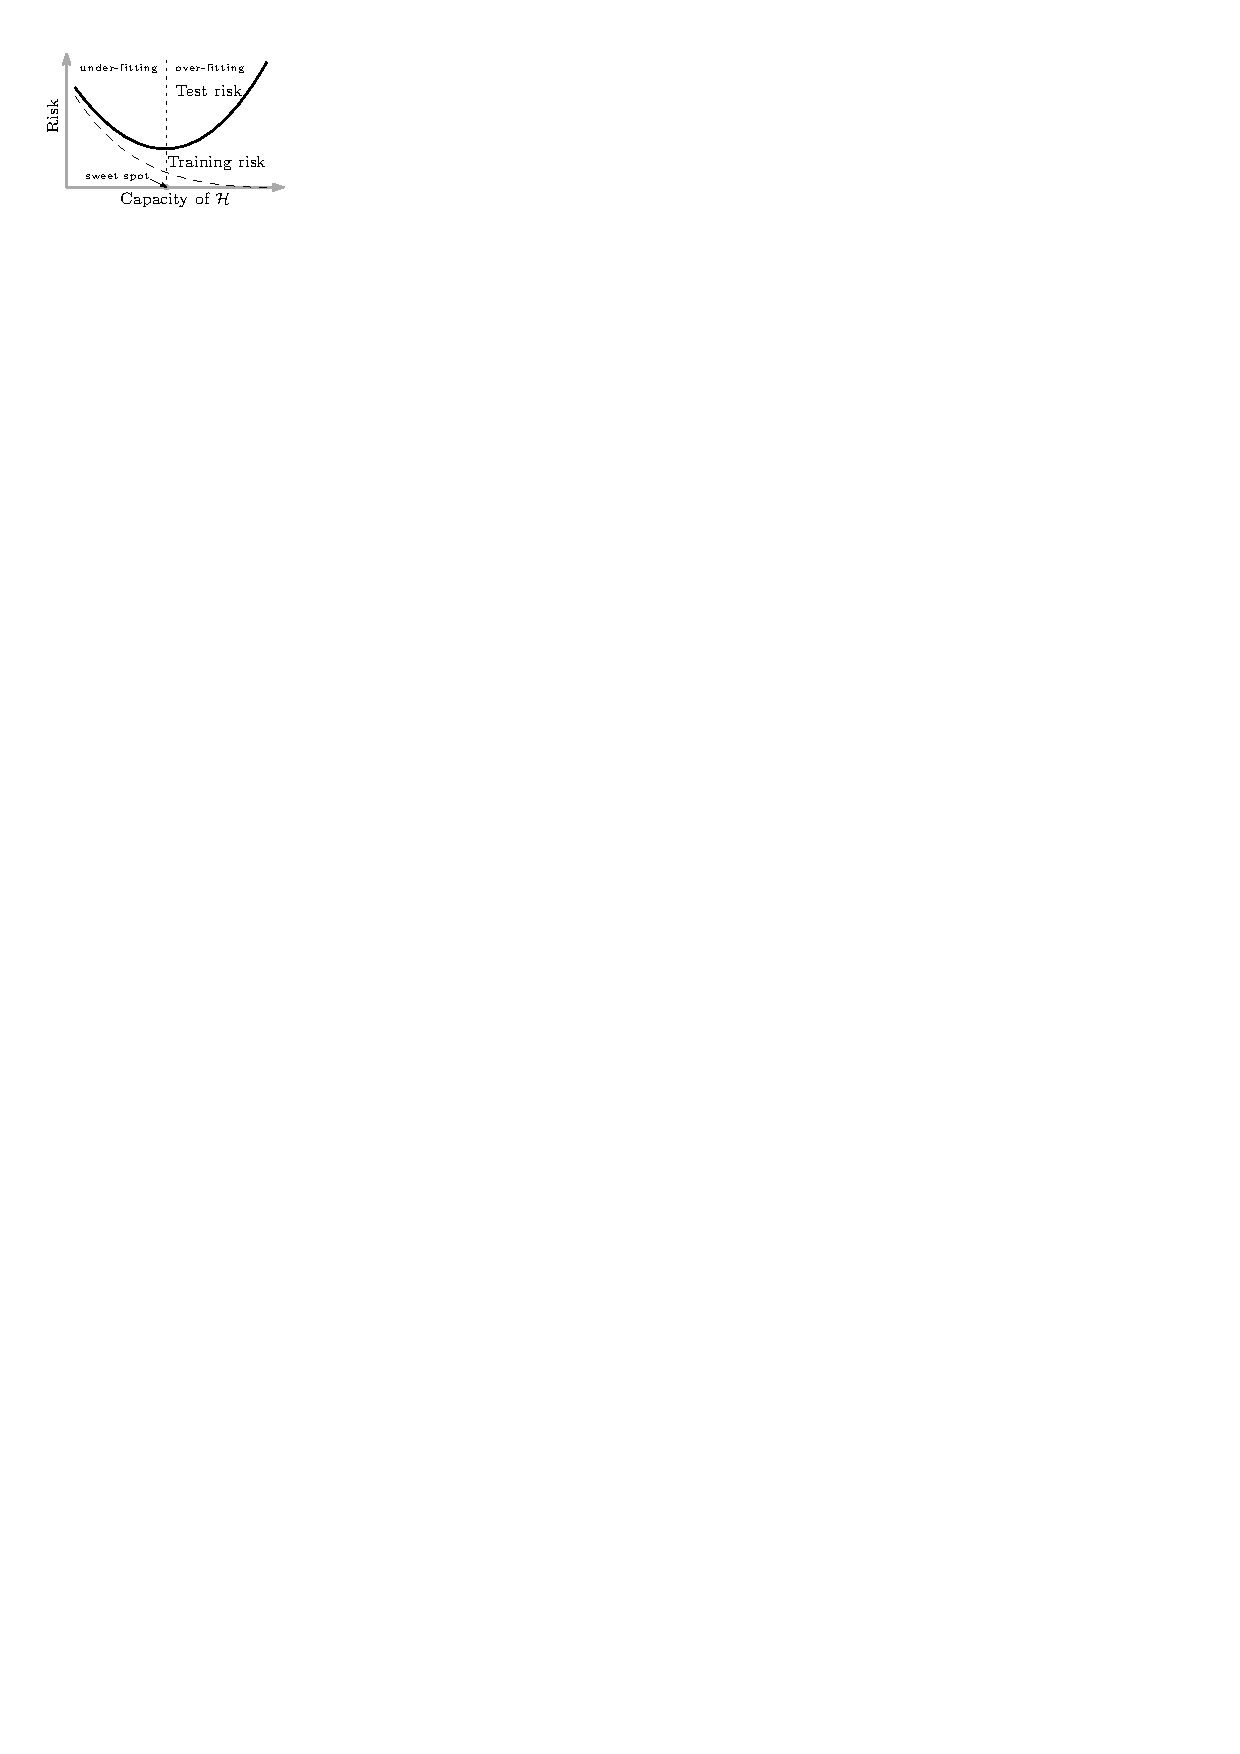
\includegraphics[height=0.13\textheight]{pdf/u-shaped.pdf} &
    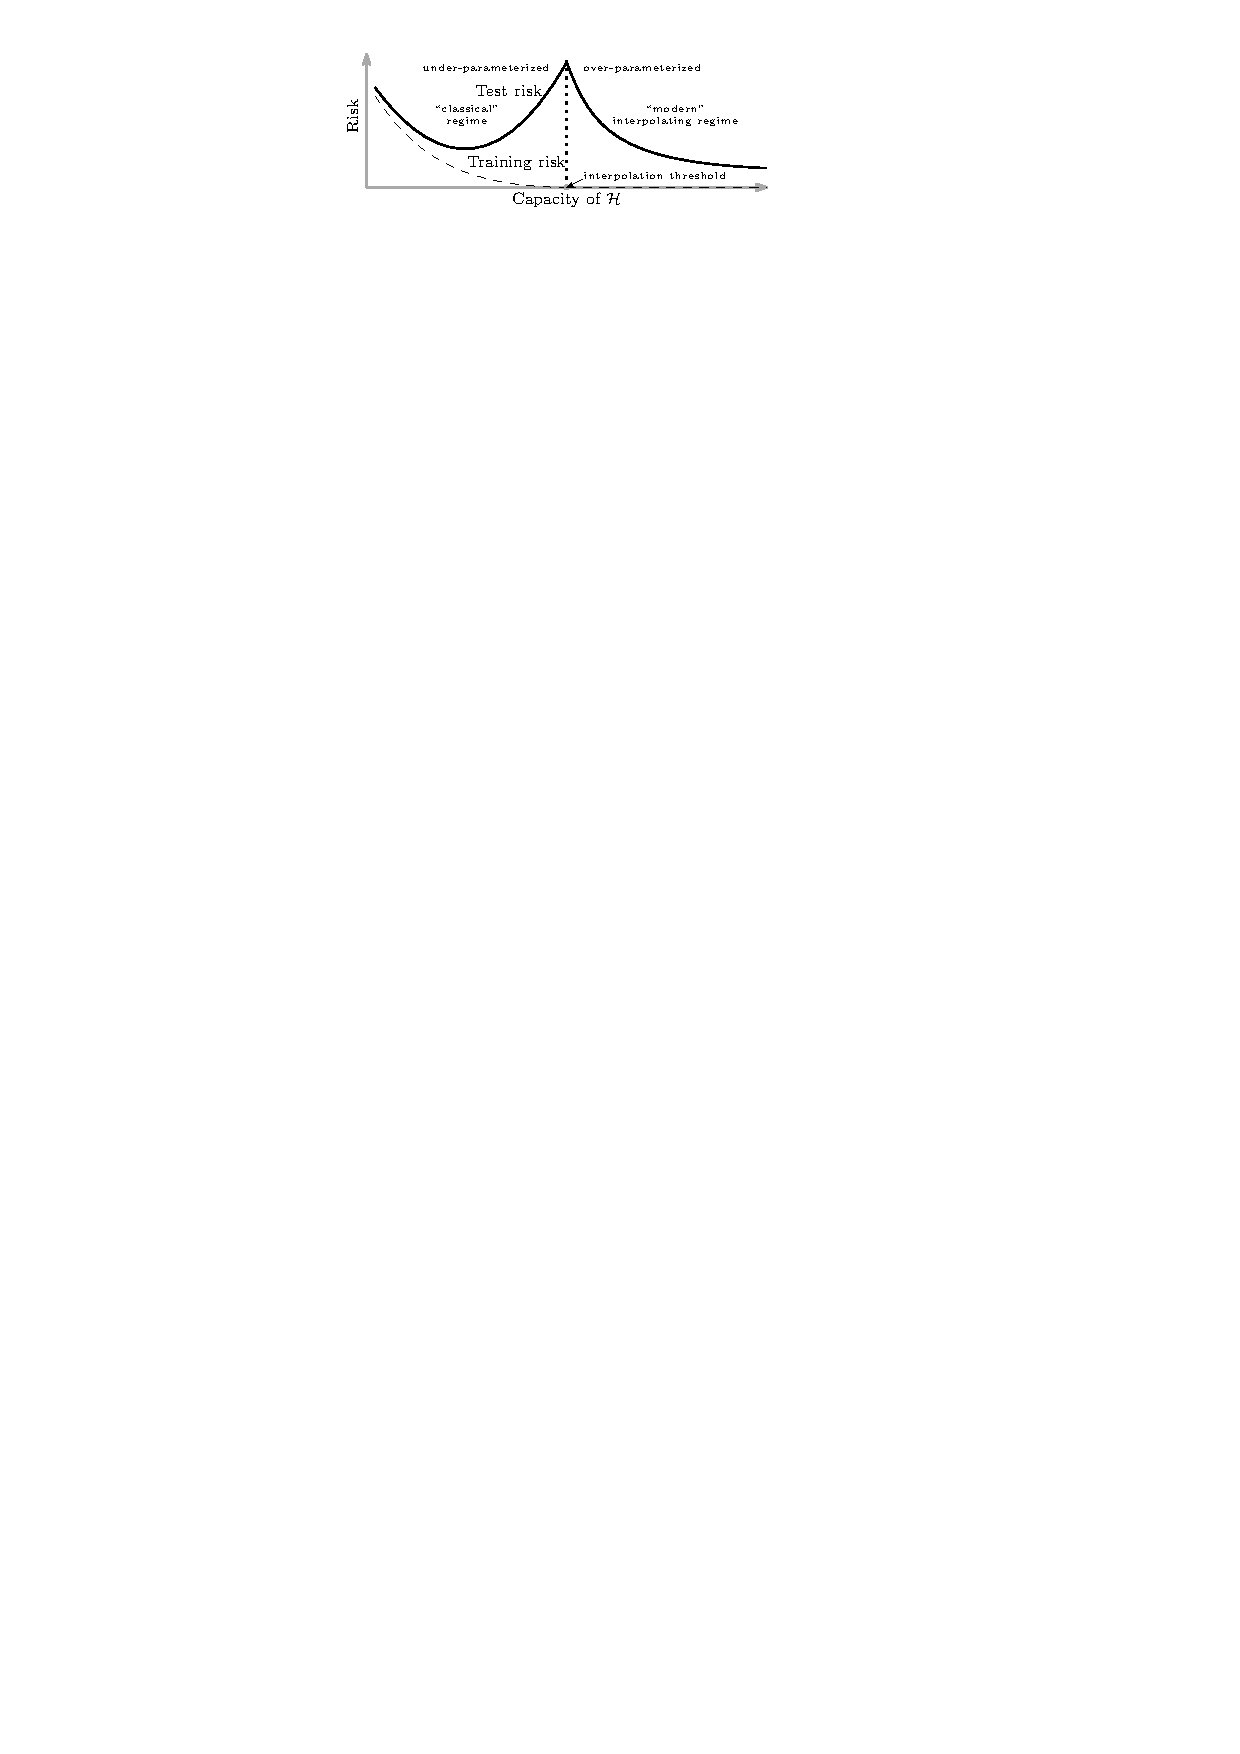
\includegraphics[height=0.13\textheight]{pdf/doubledescent.pdf} \\
    {\bf (a)} & {\bf (b)}
    \end{tabular}
    \caption{{\small {\bf Curves for training risk (dashed line) and test risk (solid line).}
      ({\bf a}) The classical \emph{U-shaped risk curve} arising from the bias-variance trade-off.
      ({\bf b}) The \emph{double descent risk curve}, which incorporates the U-shaped risk curve (i.e., the ``classical'' regime) together with the observed behaviour from using high capacity function classes (i.e., the ``modern'' interpolating regime), separated by the interpolation threshold.
      The predictors to the right of the interpolation threshold have zero training risk. Reproduced from \cite{belkin_reconciling_2019}.}}
    \label{fig:double-descent}
\end{figure*}

The main finding that Belkin found is a pattern for how the apparent performance on unseen data depends on model capacity and the mechanism underlying the emergence of double descent. When function class capacity is below the "interpolation threshold", learned predictors exhibit the classical $U$-shaped curve from Figure~\ref{fig:double-descent}. The `modern' interpolating regime marks the opposite trend to the right, where the risk starts to decrease up to a lower bound, which then can be called the \textit{optimal descent bound}. 

\blockquote[\cite{belkin_reconciling_2019}]{The bottom of the $U$ is achieved at the sweet spot which balances the fit to the training data and the susceptibility to over-fitting:
to the left of the sweet spot, predictors are under-fit, and immediately to the right, predictors are over-fit.
When we increase the function class capacity high enough (e.g., by increasing the number of features or the size of the neural network architecture), the learned predictors achieve (near) perfect fits to the training data---i.e., interpolation.
Although the learned predictors obtained at the interpolation threshold typically have high risk, we show that increasing the function class capacity beyond this point leads to decreasing risk, typically going below the risk achieved at the sweet spot in the ``classical'' regime.}

At this point, we would like to also clarify the term interpolation threshold in this case. Usually, under the pretext of overfitting and underfitting, interpolation threshold means the following: 

\begin{definition}[Interpolation threshold]
    Assuming a typical supervised learning setting, for a hypothesis $h$ within class structure $\mathcal{H}$, and a supposed concept $c$ of the class $\mathcal{C}$. Suppose $[X,Y]\subset c\in \mathcal{C}$ being the dataset, or \textit{observable space} of $c$ on which $h$ is tested on. Under the \textbf{empirical generalization learning} procedure, partitioning $[X,Y]$ into $[X,Y]_{1}$ and $[X,Y]_{2}$, for error evaluated on the first set, $\hat{R}_{1}(h)$ called training error, and the second set, $\hat{R}_{2}(h)$ called test error, with optimization applied on the first set, then evaluated statically on the second, the \textbf{interpolation threshold} with respect to a particular complexity measure of $h$, $\mathcal{M}(h)$, is the point $\mathcal{M}_{0}(h)$ where it is possible for $\hat{R}_{2}(h)/\hat{R}_{1}(h)\approx 1$, for $\hat{R}_{1}(h)\ll \epsilon$, $\hat{R}_{2}(h)\ll \epsilon$, with $\epsilon \geq 0$. 
\end{definition}

This basically means that what is learnt, with respect to the model complexity that gauge \textit{how much} and \textit{what} the model can learn, perfectly fits the concept $c$ itself, from the observation space on its own. We can say that, that specific sense, we gain the assumption that the observation space is \textit{fully representative} of the concept class, and the concept class is then fully realized by the model. Such point where that is possible, or there then such behaviour is possible, is called the interpolation point. The definition relies on the statement `where it is possible', hence it still, does not give us a particularly sound notion on to how and what constitute such possibility. The term empirical generalization learning comes from the fact that the procedure in practice of estimating and optimizing train-test-validation set in itself, is an imperfect empirical approximation of generalization testing. While the fact that we cannot gauge generalization error, in a purely blind black-box setting is settled (\cite{10.5555/2371238,10.5555/2930837,10.5555/2621980}), the method is then to try to mimic such by using generalization-via-hidden observations. To facilitate this, deliberately, the empirical learning procedure is only dynamic during training session, and static throughout the whole testing and validation testing section, and further on. 

By default, in general theory, such interpolating point is dangerous. Not only because it is inherently difficult to know exactly what the dataset constitute, whether it is actually representative of the concept that gives rise to it, or the structural information, noises, and interferences in between. It is hence impossible, to a certain point, to truly know the effectiveness of the model beside interpolating the current dataset which forms the observable details. 

Another prominent discovery to look at is \cite{nakkiran_deep_2019}, on the double descent of deep learning models. The paper serves as the first observation upon which double descent is observed on modern, deep learning theoretic models, especially complex one like Transformer or ResNet networks. They define \emph{effective model complexity} of $\mathcal{T}$ (w.r.t. distribution $\mathcal D$) to be the maximum number of samples $n$ on which $\mathcal{T}$ achieves on average $\approx 0$ \emph{training error}. This is an entirely empirical definition, similarly per definition as VC-dimension. 

\newcommand{\EMC}{\mathrm{EMC}}
\begin{definition}[Effective Model Complexity]
The \emph{Effective Model Complexity} (EMC) of a training procedure $\cT$, with respect to distribution $\cD$ and parameter $\epsilon>0$,
is defined as:
\begin{align*}
    \EMC_{\cD,\eps}(\cT)
    :=  \max \left\{n ~|~ \E_{S \sim \cD^n}[ \mathrm{Error}_S( \cT( S )  ) ] \leq \eps \right\}
    \end{align*}
    where $\mathrm{Error}_S(M)$ is the mean error of model $M$ on train samples $S$.
\end{definition}

Using this definition, their main hypothesis can then be stated as the following three-fold regions:

\begin{hypothesis}[Generalized Double Descent hypothesis, informal] \label{hyp:informaldd}
For any natural data distribution $\cD$, neural-network-based training procedure $\cT$, and small $\epsilon>0$,
if we consider the task of predicting labels based on  $n$ samples from $\cD$ then:
\begin{description}
    \item[Under-parameterized regime.]  If~$\EMC_{\cD,\epsilon}(\cT)$ is sufficiently smaller than $n$, any perturbation of $\cT$ that increases its effective complexity will decrease the test error.
    \item[Over-parameterized regime.] If $\EMC_{\cD,\epsilon}(\cT)$ is sufficiently larger than $n$,
    any perturbation of $\cT$ that increases its effective complexity will decrease the test error.
    
    \item[Critically parameterized regime.] If $\EMC_{\cD,\epsilon}(\cT) \approx n$, then
    a perturbation of $\cT$ that increases its effective complexity
    might decrease {\bf or increase} the test error.
\end{description}
\end{hypothesis}

It is to notice that this definition is also only observational. By that, it only outlines the specific region of interest where the paradigm shift is identified through experimental results. It has no effective predictive power, or rather descriptive power more than setting up hypothesis with respect to the effective model complexity, and some arbitrary perturbation. \cite{nakkiran_deep_2019} also noticed this difficulty in providing a theoretical definition and theorem regarding such hypothesis, as said in their manuscript. The existence of the critical regime is also not defined. 

The behaviour itself has been particularly investigated, in certain settings. For example, before \cite{belkin_reconciling_2019}, \cite{advani2017highdimensionaldynamicsgeneralizationerror} investigated the generalization error in neural networks of high-dimensional measure. Of such, various behaviours that bear similarity to double descent can be observed. \cite{belkin2018understanddeeplearningneed} expanded on his previous research on the particular subset of kernel learning models, providing a theoretical analysis of specifically the Laplacian kernel on standard neural network. \cite{mei2020generalizationerrorrandomfeatures} investigated random feature regression in such regard, and also found similar results. 

The fact that double descent is not well-defined itself is a problem on its own. Up to the author's knowledge and of myself, there has been no effective definition or given description that outlines specifically how double descent can be structured. Instability in reproducing experiments and the effective range of the phenomena remains a question on its own. 

\section{The polynomial transition problem}

Polynomial space is one of those famous example that is often cited of the bias-variance tradeoff, for example, in \cite{goodfellow2016deep,10.5555/2930837}. Indeed, it is considered, usually, a very effective and high-volatility construct class. Let us reiterate what we know about polynomial class. 

There exists two type of elementary polynomial classification, based on their (i) variable count or (ii) its domain range. We first define the univariate polynomial function.

\begin{definition}[Univariate polynomial]
    A function of a single variable $t$ is a polynomial on its domain if we can put it in the form 
    \begin{equation}
        a_{n}t^{n} + a_{n-1}t^{n-1} + \dots + a_{1}t + a_{0}t^{0}
    \end{equation}
    where $\{a_{i}\}$ are constants, and of a singular variable $t$.  
\end{definition}

From this, we can extend to polynomial of multiple variables. In general, a function $f(x,y)$ is a \textit{multivariate polynomial} in $x,y$ if and only if it can be represented as a finite sum of terms of the form $cx^{k}y^{m}$, where $c$ is a coefficient and $k$ an $m$ are nonnegative integers. The number $k+m$ is called the degree of the term, and the degree of the polynomial $f(x,y)$ is equal to the highest degree of its own terms. We can then generalize multivariate polynomial and univariate polynomial in the same kind. 

\begin{definition}[Polynomial, multivariate generalization]
    Let $K$ be a field. We then denote $K[x_{1},\dots,x_{n}]$ the space of all polynomials in $n$ variables, $x_{1},\dots,x_{n}$. A \textbf{multivariate monomial} is then an expression $x_{1}^{\alpha_{1}}\dots x_{n}^{\alpha_{n}}$ where $\alpha_{1},\dots,\alpha_{n}$ are integers. The degree ò such multivariate polynomial is the largest degree of terms of any monomial term.
\end{definition}
Effectively, we can see that multivariate polynomial can take on many forms, and also unconventional forms. In order to capture any reasonable details, most of the time focus are on symmetric polynomials $f(x,y)$ in which $f(x,y)=f(y,x)$, or homogeneous polynomials in which all the terms are of the same degree. 

Given such, operationally, polynomial is used for expressing other functions, due to their usefulness because of such simplicity and versatility. In fact, applications ranges, even to a polynomial basis on $n$-dimensional space, $(p_{1},\dots,p_{n})\in K[x,\dots,x_{n}]$; their growth rate being polynomial also added more to their strength of approximating fast increasing function, usually expressed and used in setting, for example, polynomial growth class $\mathcal{O}(p(x))$ in computer science. Two applications stand out for such properties: function approximation of arbitrary criteria $\ell$, or polynomial interpolation on arbitrary points. Those two are interconnected, though their objective and object of concern is much different. 

We can define the application of analytical polynomial on arbitrary function by using the criteria on approximation. Usually, this is expressed in the theory of approximation, and requires a guarantee that polynomial can indeed approximate to arbitrary accuracy, of arbitrary function on specific interval. This is the statement of Weierstrass theorem. 

\begin{theorem}[Weierstrass Approximation Theorem]
    Let $f\in C[a,b]$ of all continuously differentiable functions on the closed interval $[a,b]$. Then, for every $\epsilon > 0$, there is a polynomial $p$ such that $||f-p||< \epsilon$, for $||f-p||=\sum_{i=1}^{\infty}|(f(x_{i})-p(x_{i}))|$ \footnote{We again note the disparity between $h(x)-c(x)$ or $c(x)-h(x)$ for clarity. In essence, $c(x)-h(c)$ is looking from the perspective of the concept itself. While $h(x)-c(x)$ is comparison on difference from the perspective of the hypothesis.}
\end{theorem}
Here, $\epsilon$ is defined to be the \textit{global error} of the polynomial with respect to the arbitrary function, and with uniform approximation. Another variation works on the squared error, such that $||f-p||=\sum_{i=1}^{\infty}(f(x_{i})-p(x_{i}))^{2}$, or the mean absolute $$||f-p||=\lim_{n\to\infty}\frac{1}{n}\sum_{i=1}^{n}(f(x_{i})-p(x_{i}))$$
Weierstrass Approximation Theorem provides tighter bound for the mean absolute error, but not the square error, or the mean square case. Nevertheless, they are natural measure on the uniform metric space $C(X)$ with measure $d(f,g)=\sup_{x\in X}|f(x)-g(x)|$. If said metric also use the $L^{p}$ metric instead, which is defined by 
\begin{equation}
    d_{p}(f,g) = \left(\int_{X}|f(x)-f(g)|^{p}\:dx\right)^{1/p}
\end{equation}
we can also see that it is weaker than the bound given by Weierstrass theorem. Generalization of Weierstrass theorem can be made by Stone-Weierstrass theorem instead, of which is state in real space as followed, though generally Weierstrass theorem is sufficed.
\begin{theorem}[Stone-Weierstrass Theorem (real version)]
  Let $S$ be a locally compact Hausdorff space. Let $A$ be the subset of bounded continuous real functions on $X$, or of subalgebras $\mathcal{C}(X,\mathbb{R})$ which contains a non-zero constant function, then $A$ is uniformly dense in $\mathcal{C}(X,\mathbb{R})$ if and only if it separates points. 
\end{theorem}
The setting of polynomial interpolation is rather different from the setting of function approximation. The setting of interpolation gives an $n$ samples set $\mathcal{S}$, of which in this case we restrict to $\mathbb{R}\to\mathbb{R}$. Then, we are required to fit exactly the entire dataset, such that the following setting is sufficed. 
\begin{definition}[Interpolation]
    A function class $\mathcal{F}$ is said to \textbf{interpolate} a distinct dataset $\mathcal{S}_{n}=(x_{n},y_{n})$ of $n$ samples, if there exists $f\in \mathcal{F}$ such that $\mathbb{E}||S_{i}-|f(x_{i})||= 0$. Such $f$ is then called the \textbf{interpolating function} of $\mathcal{S}_{n}$. 
\end{definition}
Under such definition, the question is then if the polynomial class $\mathcal{P}_{n}$ of any given polynomial with the highest degree $n$ is sufficed to approximate such dataset. The answer can be found using unisolvence theorem.

\begin{theorem}[Unisolvence theorem]
    Given $n+1$ bivariate data points $(x_{0},y_{0}),(x_{1},y_{1}),\dots,(x_{n},y_{n})\in \mathcal{S}_{n}\subset \mathbb{R}^{n}$, with all $x_{i}$ distinct, there exists a unique polynomial $p_{n}(x)$ of degree at most $n$ such that $p(x_{i})=y_{i}$ for $i=0,1,\dots,n$.
\end{theorem}

In determining such problem, we can also say that there exists a unique $n$-saddle point function represented here as polynomial, such that to fit $n$ points perfectly by the definition of the saddle point. The process in obtaining such formula is difficult, however, and finding the perfect interpolation polynomial would be computationally significant, and erroneous. 

\begin{definition}[Saddle point,\cite{NieYangZhou2021}]
    Let $X\subseteq \mathbb{R}^{n}$, $Y\subseteq \mathbb{R}^{m}$ be two sets (for dimension $n,m>0$) and let $F(x,y)$ be a continuous function in $(x,y)\in X\times Y$. A pair $(x^{*},y^{*})\in X\times Y$ is said to be a saddle point of $F(x,y)$ over $X\times Y$ if \begin{equation}
        F(x^{*},y) \leq F(x^{*},y^{*})\leq F(x,y^{*}), \quad \forall x\in X, \forall y\in Y
    \end{equation}
\end{definition}

Polynomial regression is one such analytical solution to function approximation task, using Weierstrass theorem as its basis. From such, we can also observe that polynomial regression, and hence polynomial interpolation, are correlated and can be reduced to each other. Polynomial regression can be reduced to interpolation via stating the criteria such that, denoting it as $\ell$, then $\ell(f,p)=0$, and interpolation can be reduced to regression via the condition that $p(x_{i})-y_{i}\leq \epsilon$ for arbitrary $\epsilon>0$. Hence, the regression formulae lie between the two extreme: the Weierstrass setting and the interpolation setting. 

We then have to identify such extreme and what kind of extreme they represent. Fortunately, we know this as the problem of \textbf{transparency}, in the setting of approximation, which certainly correlates to the learning theory. According to such, the Stone-Weierstrass represents the total transparency case, where the function $f$ is known to the approximator with polynomial class. Interpolation represents total black box, where the goal is only to interpolate the sample point by itself. In between such interpretation, there exists a fundamental assumption, hence the structural assumption. 

\begin{assumption}[Transparency]
    For any bivariate pair $(x,y)$, we assume each pair depends on and originate from a based concept $y=f(x)$. 
\end{assumption}

Two kinds of knowledge is then available, which correlates to the degree of freedom the observation space can have. First is the knowledge of $f$. This knowledge of $f$ is encoded directly by the number of sample point and their distribution in certain case. Accordingly, the worst case is as followed. 

\begin{conjecture}
    If $\forall x$ there exists $y$ corresponding to such, and $(x,y)\in \mathcal{S}$, then we say we have total transparency to the concept $f$. If there exists only finite $x$ that we can have $y$ corresponding to, then we say we have limited transparency to the concept $f$. If we assume no knowledge of $f$, then we say the setting is called the \textbf{black-box setting}. 
\end{conjecture}

Secondly is the action on the dataset itself. One of the main assumption that is usually observed is that 

\begin{assumption}[Fallacy]
    We assume every bivariate pair $(x_{i},y_{i})\in f[\mathcal{S}_{n}]$, such that $f(x_{i})=y_{i}$. 
\end{assumption}

However, usually, this is not the case, as we have \textbf{noise} in addition from the dataset. The origin of the noise cannot be tracked. However, we can interpret what happens when such noise is introduced to the dataset. The noise transitions the transparency of the learned setting, on the field $\mathbb{R}$, by utilizing the dense property of the real space. Assuming we operate on $\mathbb{Z}$. Then, each discrete noise will introduce abnormality point such that no function on $\mathbb{Z}$ will be able to match, up to certain distance on $\mathbb{Z}$. This is because on such space, there exists no point $x_1, x_{2}$, for example, that lies between $d(x_{1},x_{2})=1$. If the noise is randomized on $\pm 1$, then there will exists no function that can approximate such disparity better than a random fluctuating function. However, on $\mathbb{R}$, the real number is inherently dense, such that there will always be certain point $x_{3}$ such that $x_{3}\in [x_{1},x_{2}]$, by the density of real number. By the distance metric on $\mathbb{R}$, we define $d(X,Y)=|X-Y|$ for distance between two data points. Noise intrinsically increases such distance, such that $d'(X,Y)> d(X,Y)$. Hence, the space in which density can appear increase, thus there then exists more fluctuation, and thus more uncertainty between such two points. This notion can be increased from local uncertainty to global uncertainty, hence the \textit{noisy dataset}. 

We then can measure or aggregate some properties of the dataset itself, including the \textbf{uncertainty} of the dataset. We define the simple uncertainty of the dataset as followed. 

\begin{definition}[Dataset uncertainty]
    Given a closed interval $[a,b]$, for the sample set $\mathcal{S}_{n}=(X,Y)\in [a,b]$, the uncertainty $\mathcal{U}(\mathcal{S}_{n})$ is defined as 
    \begin{equation}
        \mathcal{U}(\mathcal{S}_{n}) = \left[ \underset{x_{i}\in X}{\mathbb{E}}\Big( x_{i+1} - x_{i} \Big)^{2} + \underset{y_{i}\in Y}{\mathbb{E}} \Big( y_{i+1}- y_{i} \Big)^{2} \right]^{1/2}
    \end{equation}
    We assume $X,Y$ are totally ordered sets. 
\end{definition}
Hence, the assumption of fallacy assumes $\mathcal{U}(\mathcal{S}_{n})=0$, though in reality it is often $\mathcal{U}(\mathcal{S}_{n})>0$. With this, we can quantify how the dataset is behaving on the scale of the bivariate form typically seen. Noise intrinsically increases this distance, usually by the $y$-axis. This dataset uncertainty increases with multivariate dataset, for example, $(\mathbf{x},y)$ of $\mathbb{R}^{n}\to\mathbb{R}$. We call the new metric as the \textit{empirical uncertainty metric}. From this, we can have the theorem:

\begin{theorem}[Uncertainty tradeoff]
    
\end{theorem}

Thirdly, is the treatment on such information. Even though information is known, such as from the assumption of transparency and the fallacy conjecture, it relies on the method in which the model uses that make use of such information. Polynomial interpolation effectively removes information about transparency, and thus the interpolation setting is a kind of \textbf{black-box absolute setting}. This setting is \textit{extremely brittle}, as to see that if $y_{i}$ is slightly wrong due to measurement noise, the interpolant oscillates wildly, which is explained by Runge phenomenon (\cite{Runge1901,CorlessSevyeri2018,AMC2009RungeDivergence}). Probability then arises from such setting naturally, though this particular degree of probabilistic setting must be quantified, which comes from the process that the model simulates upon. Regression is inherently not probabilistic, but treatment about the probabilistic assumption, for example, such that $(X,Y)$ inherently as random variables. We can then separate this into three parts - the data-level probabilistic layer (data uncertainty), the model-level layer, and the algorithm-layer that determines the solution solver within such model. We can define that as followed. 

\begin{definition}[Probabilistic layer]
    Given a learning setting with dataset $\mathcal{S}$ of bivariate pairs, $h\in \mathcal{H}$, $c\in \mathcal{C}$ as the hypothesis and concept, we have the following conceptual probabilistic setting:\footnote{Currently, we have no way to \textbf{quantify} the `probabilistic degree' of the system setting itself}
    \begin{enumerate}
        \item Data-level probability: Sampling assumptions (observation sample points) such that there exists the distribution $\mathcal{D}\sim (X,Y)$, intrinsic data uncertainty $\mathcal{U}(\mathcal{S}_{n})$. 
        \item Model-level probability: Structure of the dataset is controlled by the concept structure $\{\theta\}\in c$, $c$ is modelled as a target sampler $c\equiv \mathcal{D}$, knowledge about the structure of $c$, Bayesian prior-posterior assumptions, $\mathbb{P}(Y\mid X, \{\theta\})$. For Bayesian polynomial regression, the model-level probability is formulated as \begin{equation}
            \mathbb{P}(Y\mid X) = \int \mathbb{P}(Y\mid X,\theta)\mathbb{P}(\theta)\: d\theta, \quad \mathbb{P}(\theta_{j}) = \mathcal{N}(0,\sigma^{2})
        \end{equation}
        of which assumes aleatoric uncertainty and epistemic uncertainty from the weight. 
        \item Algorithm-level probability: Stochastic method, decision conditional (dropout, MCMC), ensembles criteria, Monte-Carlo initialization, variational inference. 
    \end{enumerate}
\end{definition}

Dynamically, in this paper, we would like to investigate this particular junction between uncertainties, to see what happens when the model transparency, the treatment of data, and so on, that exhibits the observations that we would receive from the model itself. The experimental details will infer such result. 

Generally, we would be entitled to see particular trajectory specifically designed around the point of interpolating match, or $n=m$ of $n$ degree of freedom, technically, and $m$ data points. After this point, there exist two possibility of dynamic - either the model dilutes, in which case result in \textit{double descent}, or the model fluctuate strongly afterward, leading to \textit{bias-variance emergence} again later on. This conclusion however, would have to be analysed within the current framework of the possible interjection to its fluctuation strength. For example, in the monomial basis $\{x^{i}\}^{n}$, any given fluctuation contributes to the entire polynomial. In such case, fluctuation of the other $[0,n-k]$ of arbitrary $k$ and large enough $n$ would be unaccounted for by the scale. Conversely, restrict them to $[1,0]$ range will reveal something about the system, however will destroy particular properties of the prediction, which is not recommended. Nevertheless, we must conduct the test before giving in any reasonable conclusion.

Previously, we said that we did indeed focus on the interpolation problem. Now, assuming we have given the interpolating algorithm $\mathcal{A}$ to approximate the interpolation, what will this look like? Firstly, solving this is \textit{very computationally expensive}, because it is a dense, $(n+1)\times(n+1)$ linear system, and even more so if we consider the overparameterized outcome. However, this can be reduced further down if we attempt to solve them using convergence bound, but will be still very expensive. That and incremental soft interpolation is somewhat out of the question since it will be kind of the same. Aside from the insight, we would still have to know what to do. Then there exists two ways - we have some version of this to optimize of simply evaluating by gradient descent optimization, or, we can use somewhat analytical fit for the case of soft interpolation modification. 

A theory on such problem can be obtained of its mechanics, as will be a fairly intuitive way in consideration of the theory of interpolation, as well as the technique of interpolation by itself. For a fixed-range interpolation threshold problem, a hard-encoded interpolation solution requires $n$-degree polynomial, of which has $n+1$ degree of fitness, to fit $n+1$ distinct points. Suppose all points are distinct of the set $S$ which is finite, then this is the case. If we switch to the problem of interpolation but induce a more forgiving bound, there exists a possibility that it induces a relative \textit{density averaging path} for the points, especially if we are considering the case where $p>n$ for $p$ saddle points or degree of fitness, and $n$ the number of point to interpolate. In a more nuanced formulation, we have

\begin{equation}\label{eq:soft_hard_interpolation_role}
\mathsf{Flatten}\left(\begin{bmatrix}
1 & x_0 & x_0^2 & \cdots & x_0^p \\
1 & x_1 & x_1^2 & \cdots & x_1^p \\
\vdots & \vdots & \vdots & \ddots & \vdots \\
1 & x_p & x_p^2 & \cdots & x_p^p \\
\vdots & \vdots & \vdots & \ddots & \vdots \\
1 & x_n & x_n^2 & \cdots & x_n^p
\end{bmatrix}_{n\times p}
\begin{bmatrix}
a_0 \\
a_1 \\
a_2 \\
\vdots \\
a_p
\end{bmatrix}
- 
\begin{bmatrix}
f(x_0) \\
f(x_1) \\
f(x_2) \\
f(x_3) \\
\vdots \\
f(x_n)
\end{bmatrix}\right)
\leq \epsilon
\end{equation}
or equivalently, $\mathsf{Flatten}(\mathbf{X}_{n\times p}\mathbf{w}_{n}-\mathbf{Y}_{n})\leq \epsilon$ where $\mathsf{Flatten}(\cdot)$ is the compression of vector to scalar, or so $\mathsf{Flatten}: \mathbb{R}^{n}\to \mathbb{R}$. This essentially is the problem of solving $n$ points approximation, toward using only $p$ saddle points available. If $\epsilon =0$, it is well known that interpolation is impossible. However, if $\epsilon\ne 0$, there are possibilities, depends on the shape of the dataset, that there will exist a data-dependent property or more that indict a particular \textit{density preference} toward those saddle points - or rather, the act of density averaging. This is reflected rather implicitly in the structure itself. In machine learning, the error measure is usually the mean average, such is to say that the criterion now would look more like $\mathbb{E}\Big[\mathsf{Flatten}(\mathbf{X}_{n\times p}\mathbf{w}_{n}-\mathbf{Y}_{n})\Big]\leq \epsilon$. Formally, we have the following hypothesis

\begin{hypothesis}[Polynomial double descent]\label{hyp:hypothesis_poly_dd}
For a polynomial $\{a_{i}x^{i}\}_{n}$ on Vandermonde basis, approximating on the set $\{(x_{k},y_{k})\}_{m}$, then
\begin{enumerate}[topsep=1pt,itemsep=1pt]
  \item For $n<m$, we expect the polynomial form factor to be \textit{inherently sparse}, such that for an iterative approximation, for each $p_{i}$ saddle point of the polynomial expansion form, there exists an $\epsilon$-ball $B_{\epsilon}$ for $\epsilon>0$ with at least one data point satisfying $(x_{k},y_{k})\in B_{\epsilon}$. 
  \item For $n=m$, we expect the polynomial to be able to fit all points, up to hard interpolation threshold such that $\hat{R}_{S}\approx 0$. 
  \item For $n>m$, we expect the polynomial form factor to be \textit{locally dense} then turning to \textit{globally dense}, over random ensembles. That is, for every point $(x_{k},y_{k})$ there exists a $\beta$-ball $B_{\beta}$ such that there is at least one saddle point of the polynomial belong to the ball. 
\end{enumerate}
\end{hypothesis}

The shift that will be hypothesized to appear here is expected to be from sparse in the polynomial term sense, out to globally dense with enough model complexity, over an iterative process. One also main point of clarity is, at certain point right now, we haven't discovered the effect of error deviation, yet. For such, we theorize the following. 

\begin{conjecture}[Double descent]
  Double descent happens, for a polynomial class model $h_{n}\in\mathcal{H}_{p}$, is upper bounded to certain error deviation $\epsilon>0$ from the mean only of the generalization (test) dataset verification. 
\end{conjecture}

\begin{figure}[htb]
  
\includegraphics[width=\textwidth]{diagram_poly_dd.png}
  \caption{\small\textbf{Intuition of Hypothesis~\ref{hyp:hypothesis_poly_dd}}. Effectively, in the overparameterized range $(p>n)$, the problem turns into soft interpolation, where the polynomial is possible to be dense enough such that relative error remains internally low. This can also happen if the dataset itself is intrinsically large.}
\end{figure}

That is, the disparity between the test and training dataset helps in such regard. If the two dataset is partitioned in the sense that their deviation is practically the same (which can be done using synthetic generation for a control group), then this will amount to not much of it. After all, it will be the consequence of the algorithm and error landscape interpretation used. 

For this, we propose another speculative observation beside such, as to consider adjourned transform of the Vandermonde basis to the Newtonian or similar basis, in which the effects and motion can be easily observed, as least easy. This is because aside from mapping down to $[-1,1]$, normal polynomial on monomial basis gives suboptimal result because of intrinsic high-degree term domination. This will become more relevant later on in the analysis. 

\subsection{Structure}

For mathematical analysis and experimental design, we would like to state the current main structure of a polynomial model. Specifically, in such example, we are concerned of the shallow polynomial neural network, of which is stated as such in \cite{arjevani2025geometryoptimizationshallowpolynomial}. Notice that it is defined on the normal Vandermonde basis, where an expression of such polynomial model under Newtonian or Lagrangian basis is not so clear-cut of an analysis. 

\begin{definition}[Shallow polynomial neural network]\label{def:poly_structure1}
    A shallow polynomial is a neural network of one layer that are functions $f_{\mathcal W}$, defined such as:
$\mathbb R^d \rightarrow \mathbb{R}$ of the form
\begin{equation}\label{eq:network_model} 
    \begin{split}
        &f_{\mathcal W}(x) = \sum_{i=1}^r
\alpha_{i} (w_i \cdot x)^d,\\  
&\mathcal W = (\alpha,w_1,\ldots,w_k) \in
\mathbb{R}^r \times (\mathbb{R}^{n})^k,
    \end{split}
\end{equation} 
where $d \in \mathbb{N}$.
\end{definition}

A modification is then available, in which we simply add $b(\cdot)$ for random initialization process. We note that this introduces certain flexibility to the model initial interpolation curvature.   
\begin{definition}[Polynomial neural network, general]\label{def:poly_model_test}
    The polynomial network based on Model~\ref{def:poly_structure1} is modified as 
    \begin{equation}
        f_{\Theta}(x) = \sum_{i=1}^{d} \theta_i \left( \mathbf{w}^\top x \right)^i + b,
    \end{equation}
    where $\Theta = (\{\theta_{i}\},\{w_{k}\},b)$.
\end{definition}

From this, we can state the model within a testing scenario listed as such, to fully capture the structural foundation of the related testing model class. For the notion of complexity, naively, we employ two kinds of complexity measure. First is the usual complexity measure via parameter counts. Second, is the expressive complexity on the basis of the linear transformation space. That is, an expressive complexity that take into account the fact that $\mathcal{O}(wx^{n})$ will always be stronger than $\mathcal{O}(wx^{n-1})$ for $x>1$. All of which can be contained in a singular expression, as seen in definition~\ref{def:pec}. However, we would have to analyse what is happening inside the metric itself. The model itself is illustrated in Figure~\ref{fig:plm}.

\begin{table*}
  \centering
  \footnotesize
  \begin{threeparttable}
    \caption{Controllable parameters and hyperparameters for polynomial class analysis}
    \label{tab:polynomial_test}
    % three columns: adaptive widths
    \begin{tabularx}{\textwidth}{ L{0.25\textwidth}
                                     L{0.2\textwidth}
                                     >{\RaggedRight\arraybackslash}X }
      \toprule
      \textbf{Information} & \textbf{Notation} & \textbf{Details} \\
      \midrule
      Hypothesis model
        & $h[\mathcal{W}_{h},\mathbf{H}_{h}]\in \mathcal{H}$
        & Hypothesis model. For simplicity, it contains $\mathcal{W}$ as the configuration parameter set, and $\mathbf{H}$ the fixed hyperparameters \\
      \addlinespace[1pt]
      Concept model
        & $c[\mathcal{W}_{c},\mathbf{H}_{c}]\in \mathcal{C}$
        & Concept or target model. Similar configuration as the hypothesis model \\
      \addlinespace[1pt]
      Complexity measure(s)
        & $\{\mathbb{C}(\cdot)\}$
        & Set of complexity measure of choice for any arbitrary model taken in. \\
      \addlinespace[1pt]
      Sample count
        & $m$
        & The number of sample available for hypothesis model of $c$, for $m=|\mathcal{S}|$ dataset\\
      \addlinespace[1pt]
      Hypothesis dimension (hyperparameter)
        & $[d_{h}]$
        & An explicit hyperparameter contains the list of all in-testing polynomial degree for the hypothesis model. \\
      \addlinespace[1pt]
      Concept dimension (hyperparameter)
        & $d_{c}$
        & An explicit hyperparameter of the concept's true dimension. Theorized such that $d_{c}=d_{h,i}$ for arbitrary $i$ will reduce to possible low-error problem.\\
      \addlinespace[1pt]
      Data noise
        & $\epsilon_{\mathcal{S}}$
        & Dataset-wide noise with relative strength to the value of the sample point. This is to reduce vanishing noise with higher-degree polynomial sample points. \\
      \addlinespace[1pt]
      Learning parameters
        & $\mathrm{epoch}, lr, \mathrm{bs}$
        & Two main parameters for gradient-descent, iterative-based algorithm - the epoch, the learning rate, and the batch size.\\
      \bottomrule
    \end{tabularx}

    \begin{tablenotes}
      \footnotesize
      \item[] \textbf{Notes:} We output to $\{\mathbb{E}[\ell]\}$ as the expected value of the error measure on $h,c$. There are a few things possible, but under approximation setting, we use MSE-on-parameter and MSE-on-prediction for two different insights: internal representation and external representation. 
    \end{tablenotes}
  \end{threeparttable}
\end{table*}

\begin{figure}[htb]
    \centering
    
\includegraphics[width=0.9\linewidth]{diagram_poly_model.png}
    \caption{Illustration of polynomial model in definition~\ref{def:poly_model_test}.}
    \label{fig:plm}
\end{figure}

In the equation for expressive complexity, the first term is the normalized linear parameters $\theta_{i}$ fixing and controlling the shift of the polynomial inning parameter, the second term is the sum of weight-aware complexity with degree factor, and the degree factor over operating range $||x_{max}-x_{min}||$ of the dataset, for the degree complexity. The final term is the last weight-aware complexity for the dominating degree $n$ of the polynomial function. Let us begin with the gauge on coefficient norm, i.e. the term $||\alpha_{d}||+1$. Here, we set $1$ as baseline, and the arbitrary norm on $\alpha$ there coefficient effect. The terms coefficient in this expression matters because, for a function $f:[a,b]\to\mathbb{R}$, the Lipschitz constant $L$ for polynomial $f$ goes by 
\begin{equation}
\begin{split}
L_{p} 
&= \sup_{x\neq y}\frac{|f(x)-f(y)|}{|x-y|} \\
&= \sup_{x\neq y}\frac{|f_{\Theta}(x)-f_{\Theta}(y)|}{|x-y|}, \\
&\leq \sup_{x \in [a,b]} \| f_{\Theta}'(x) \|_2 \\
&= \sup_{x \in [a,b]} \left\| \sum_{i=1}^{d} i \, \theta_i \, (\mathbf{w}^\top x)^{i-1} \, \mathbf{w} \right\|_2 \\
&\le \|\mathbf{w}\|_2 \, \sup_{x \in [a,b]} \sum_{i=1}^{d} i \, |\theta_i| \, |\mathbf{w}^\top x|^{i-1} \\
&\le \|\mathbf{w}\|_2 \sum_{i=1}^{d} i \, |\theta_i| \, \max \{ |\mathbf{w}^\top a|, |\mathbf{w}^\top b| \}^{i-1}.
\end{split}
\end{equation}

Where we note that $f_{\Theta}(x)=\sum_{i=1}^{d} \theta_i \left( \mathbf{w}^\top x \right)^i + b$, and $||\mathbf{w}||_{2}$ is the Euclidean $\ell^{2}$ norm. The magnitude of $f_{\Theta}'(x)$ depends directly on the coefficient size $\alpha_{i}$, and also on how big is $x$ on the domain. All of this mean for large expression and value range on $f_{\Theta}$, the Lipschitz constant of that model is accordingly large. Defining $\alpha$-norm that way is a cheap proxy for Lipschitz constant, since it gauges stability, and rate of change of the functional expression itself. 

\begin{definition}[Polynomial expressive complexity]\label{def:pec}
    For $x>1$ or $\mathbf{x}_{i}>1$ of $\mathbf{x}\in\mathbb{R}^{n}$ as input. Denote the polynomial class as $\mathcal{P}_{n}$ of their highest degree $n$, then we define the total expressive complexity of $p\in \mathcal{P}_{n}$ as followed.
\begin{equation}
    \begin{split}
        &\mathbb{C}_{E}(p)\\
& \quad = \mathbb{E}\!\Bigg[
\|\alpha\|_{d} + 1\\
& \quad + \frac{\sum_{i\in S\setminus\{p_{n}\}} w_i\,i}{\|p\|-p_{n}}\\
&\quad + \frac{1}{||\overline{x}-\underline{x}||}\!\left(
\frac{\sum_{i\in S} i}{\|p\|} + w_{n}n
\right)
\Bigg],
    \end{split}
\end{equation}
    where $S=\{p_{j}\}$, $||p||$ denotes the amount of different degree separable terms and $||x_{max}-x_{min}||$ is the observable range of the dataset. 
\end{definition}

\subsection{Scenario schema}
The scenario schema will be as followed. The following set of parameters are required for controlling the testing case, aside from different system measures. For parameter error, we reuse equation from Definition~\ref{def:pec} but with degree aware terms. This is covered in Table~\ref{tab:polynomial_test}.

We note a few problems with both interpolation interpretation and polynomial regression of higher-degree terms. Firstly, is the intrinsic interpolation error and numerical, software issue error. Higher degree polynomial can be represented as solving for a wide Vandermonde system of $n$ degrees for $m$ sample points. Using monomial basis for interpolation, either for soft interpolation also exhibits instability and numerical garbage within the operations, as indicated by \cite{Shen_2025}. They can also be a potential source of double descent, as the majority of models tested around this range are not coded effectively for handling large data operations as such, and artifacts from such choices might be taken as the indication of double descent in some particular cases. 

Aside from it, and aside from the fully-connected case, we have the particular testing scenario that can be expected of the ease of implementation. First, is the mundane implementation that is of gradually increasing degree mismatch. That is, for polynomial of $h_{p}$ and $c_{p}$, one requires only $d_{h}$ and $d_{c}$ to figure out the structure as there will exist exactly $d+1$ with the constant term, terms of which of finite many degrees. The second case is where for $p$ chosen randomly, such that aside from such $p$ entry, then the other degree or nodes of input are simply scattered dependent nodes, linear algebraically. That is, for a uniformly constructed $d$-degree network, choose at random $p$ particular degree to be fixed, while the other of $d-p$ are assigned randomly of belonging to some $p_{i}\in \{p\}$ nodes given the random choice on $p$ above. Linearly algebraically, scattered and dependent nodes then mean for example, node $4$ might use node $35$'s degree, and vice versa (if they were both non-fixed). The dependency structure is deliberately randomized rather than organized. For overparameterized case, we simply design the hypothesis by the following line of justification. For a mapping $\mathbb{R}^{d}\to\mathbb{R}$, the mapping $\mathbb{R}^{d+n}\to \mathbb{R}$ for $n= 1$ requires additional information, since the source provision does not contain information to handle additional $n$ dimensional input. Hence, we design it the following. For the hypothesis $h$, such unit of which does not fit to the original input space, the \textit{internal input space} that $h$ `hypothesize' contains, for the other $n$ entries, $q\leq d$ per unit input. That is, each input of $n$ overparameterized case receives at random, $q$ inputs can be received, for example, $w_{n1}x_{j}+w_{n2}x_{k}$ for $k,j$ specific input numbering. By the simplicity argument, then $q=1$ for the simplest case. However, this creates a skewed polynomial network, of which informally, the provided structural bias or additional information, is the fact that there exists overparameterization. To prevent this, instead, the final case considers the most general structure --- for each unit, each one can take $q$ inputs controlled as hyperparameter of the network, then the set $\{p\}$ of chosen degree influence their degree choice, and is uniform if the sampling process it is not included. 

\clearpage

\nocite{*}
\printbibliography


\end{document}